\scanpage{82}
\deleted{Extensions et biextensions des groupes algébriques\inserted{\unsure{abstraits|abstrait}} par $\unsure{G_m}$}
\figure{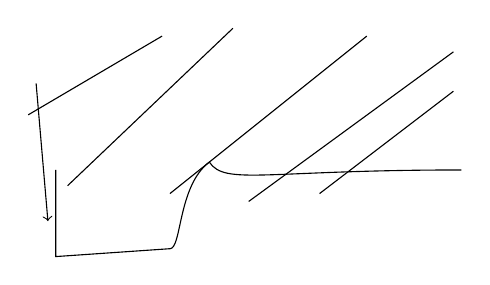
\begin{tikzpicture}[x=1cm,y=1cm]
\draw (0,2.5)--(1.7,3.5);\draw (.5,1.6)--(2.6,3.6);\draw (1.8,1.5)--(4.3,3.5);\draw (2.8,1.4)--(5.4,3.3);\draw (3.7,1.5)--(5.4,2.8);
\draw[->] (.1,2.9)--(.25,1.15);
\draw (.35,1.8)--(.35,.7)--(1.8,.8)..controls(1.95,.8)and(1.9,1.6)..(2.3,1.9)..controls(2.5,1.6)and(3,1.8)..(5.5,1.8);
\end{tikzpicture}}

Autodualité de la Jacobienne, suivant Artin-Mazur.
\mspage{81}
